\chapter{扩展不确定性精炼有序关系及其计算}\label{cha:exroru}
\section{ExRORU算法概述}\label{sec:exroru_intro}
本章主要介绍基于扩展不确定性精炼有序关系的过程模型行为语义刻画方法,即ExRORU算法(Extended Refined Ordering Relations with Uncertainty)。ExRORU算法主要包含两部分工作:一是基于CPU抽取事件间的ExRORU关系,二是将事件间的ExRORU关系折叠得到WF-net变迁之间的ExRORU关系。本章重点介绍ExRORU的定义和计算方法,其计算过程如图\ref{fig:exroru_procedure}所示。

\begin{figure}[htbp]
  \centering
  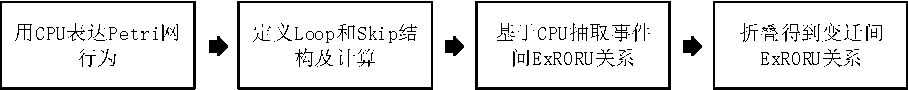
\includegraphics[width=1.0\textwidth]{exroru_procedure}
  \caption{ExRORU算法的基本流程\label{fig:exroru_procedure}}
\end{figure}

\textcolor{red}{
ExRORU计算步骤如下:
\begin{enumerate}[1.]
  \item 计算CPU。依据定义\ref{def:cpu},构造给定合理WF-net的CPU。
  \item 抽取事件间ExRORU关系。
\end{enumerate}
}

\section{事件间扩展不确定性精炼有序关系}\label{sec:exroru_event}
本节主要介绍CPU中事件间扩展不确定性精炼有序关系的定义及其计算。方便起见,约定$\Sigma=(P,T,F,M_{0})$是一个合理WF-net,$U=(B,E,A,f)$是其CPU。令$x,y\in E$是$U$的两个事件。示例WF-net及其CPU如图\ref{fig:case_study}所示。

\begin{figure}[htbp]
  \centering
  \begin{subfigure}{1\textwidth}
  	\centering
  	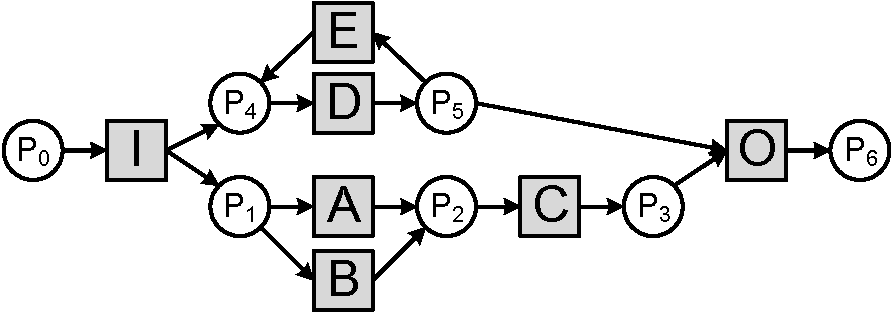
\includegraphics[width=0.8\textwidth]{case_study_petri}
  	\caption{一个合理WF-net}
  	\label{fig:case_study_petri}
  \end{subfigure}
  \begin{subfigure}{1\textwidth}
  	\vspace{1em}
  	\centering
  	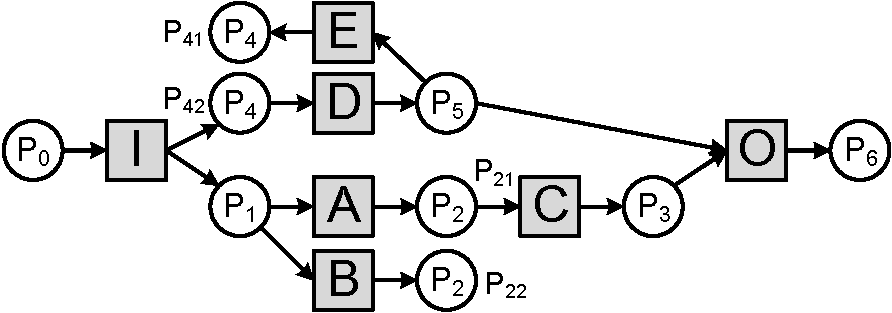
\includegraphics[width=0.8\textwidth]{case_study_cpu}
  	\caption{图\subref{fig:case_study_petri}的CPU}
  	\label{fig:case_study_cpu}
  \end{subfigure}
  \caption{一个合理WF-net及其CPU示例}
  \label{fig:case_study}
\end{figure}

\subsection{事件间扩展不确定性精炼因果关系}\label{subsec:exroru_event_causal}
本文用形如$[ab\{c,d\}e]$的表达式来描述过程流的行为语义。连续出现的字母表示处于顺序结构中的事件;大括号中的表达式表示并行结构,其不同分支用逗号隔开。该表达式可以互相嵌套以表达复杂过程流的语义。例如在图\ref{fig:case_study_cpu}的CPU中,$[I\{D,AC\}O]$、$[I\{D,BC\}O]$和$[I\{DED,AC\}O]$是一些过程流表达式示例。

轨迹是一系列事件的有穷序列$\sigma\in E^{*}$,可以从网的初始状态开始按顺序执行其中的事件最终得到终止状态。令$\Omega$是$U$中所有过程流的轨迹集合。不可见事件/变迁是模型中起路由作用的无意义事件/变迁,在逻辑流中不被表达出来\cite{wen2007mining}。本文使用带斜线的阴影方框表示不可见事件/变迁,如图\ref{fig:sda_example}所示。基于两个事件是否能在一条轨迹中紧邻发生,首先定义直接和简介因果关系。

\begin{definition}[直接和间接因果关系]\label{def:exroru_event_causal_direct}
事件$x$和$y$满足因果关系,即$x<y$。它们满足直接因果关系当且仅当:$\exists\sigma=\langle e_{1},e_{2},...,e_{n}\rangle\in\Omega,1\leq i<j\leq n,e_{i}=x,e_{j}=y$,使得$\forall k\in(i,j)$,$e_{k}$是不可见事件。否则,$x$和$y$满足间接因果关系。
\end{definition}

\begin{example}\label{ex:sda}
在图\ref{fig:case_study_cpu}的CPU中,事件$A$和$C$、事件$C$和$O$都满足直接因果关系而事件$A$和$O$满足间接因果关系。
\end{example}

令$\Uptheta$是经$U$展开得到的所有过程流集合,$\Uptheta_{x}$是$\Uptheta$中含有$x$的过程流子集,即$\Uptheta_{x}=\{\beta\in\Uptheta|x\in\beta\}$。$TS(\beta)$表示过程流$\beta$所有轨迹的集合。

\begin{definition}[事件间扩展不确定性精炼因果关系]\label{def:exroru_event_causal}
事件$x$和$y$满足:
  \begin{itemize}
  	\item[-] 总是因果关系(always causal relation),记作$x\overset{\text{\tiny{A}}}{\rightarrow}y$,当且仅当:$x<y$且$\forall\beta_{x}\in\Uptheta_{x}$,$\forall\sigma\in TS(\beta_{x})$:在$x$被执行后,$y$必须被执行且在每两个$x$的执行之间(如果$\sigma$中有超过一个$x$)至少有一个$y$要被执行。
  	\item[-] 从不因果关系(never causal relation),记作$x\overset{\text{\tiny{N}}}{\rightarrow}y$,当且仅当:$\forall\beta_{x}\in\Uptheta_{x}$,$\forall\sigma\in TS(\beta_{x})$:当$x$被执行,$y$不能在其之后被执行。
  	\item[-] 有时因果关系(sometimes causal relation),记作记作$x\overset{\text{\tiny{S}}}{\rightarrow}y$,当且仅当$x$和$y$不满足上述两种关系。
  \end{itemize}
进一步,如果$x$和$y$满足直接因果关系,则$x\overset{\text{\tiny{DA}}}{\rightarrow}y$或者$x\overset{\text{\tiny{DS}}}{\rightarrow}y$(“$D$”表示“direct”);否则$x\overset{\text{\tiny{IA}}}{\rightarrow}y$或者$x\overset{\text{\tiny{IS}}}{\rightarrow}y$(“$I$”表示“indirect”)。
\end{definition}

定义\ref{def:exroru_event_causal}中的关系统称扩展不确定性精炼因果关系(extened refined causal relations with uncertainty),用$\rightarrow$表示,本文在不引起歧义的情况下将其简称为因果关系。显然,满足“从不因果关系”的两个事件是无需区分其是否满足“直接因果关系”的。

\begin{example}\label{ex:exroru_event_causal}
在图\ref{fig:case_study_cpu}的CPU中,事件$A$和事件$C$满足“直接总是因果关系”(direct always causal relation),即$A\overset{\text{\tiny{DA}}}{\rightarrow}C$,因为在所有含有事件$A$的轨迹中两者都满足定义\ref{def:exroru_event_causal}中的条件,且它们可以被紧邻执行;事件$E$和事件$O$满足“间接有时因果关系”(indirect sometimes causal relation),即$E\overset{\text{\tiny{IS}}}{\rightarrow}O$,因为在第一次$E$被执行和$O$被执行之间可能有更多的$E$,且两者的执行之间事件$D$至少会被执行一次(不能被紧邻执行);事件$A$和事件$B$满足“从不因果关系”(never causal relation),即$A\overset{\text{\tiny{N}}}{\rightarrow}B$,因为两者不会同时在一条轨迹中被执行。
\end{example}

根据定义\ref{def:exroru_event_causal},两个事件之间的扩展不确定性精炼因果关系共有五种,分别用$\overset{\text{\tiny{DA}}}{\rightarrow}$,$\overset{\text{\tiny{DS}}}{\rightarrow}$,$\overset{\text{\tiny{IA}}}{\rightarrow}$,$\overset{\text{\tiny{IS}}}{\rightarrow}$,$\overset{\text{\tiny{N}}}{\rightarrow}$表示。在实际应用中,只有正向的因果关系往往无法完整表达过程模型的行为语义,因为两个事件的正向因果关系不确定性和逆向因果关系不确定性常常是不一样的。为了更为准确地刻画过程模型的行为语义,本文进一步引入了扩展不确定性精炼逆因果关系(extened refined inverse causal relations with uncertainty)。

\begin{definition}[事件间扩展不确定性精炼逆因果关系]\label{def:exroru_event_inverse_causal}
事件$y$和$x$满足:
  \begin{itemize}
  	\item[-] 总是逆因果关系(always inverse causal relation),记作$y\overset{\text{\tiny{A}}}{\leftarrow}x$,当且仅当:$x<y$且$\forall\beta_{y}\in\Uptheta_{y}$,$\forall\sigma\in TS(\beta_{y})$:在$y$被执行前,$x$必须被执行且在每两个$y$的执行之间(如果$\sigma$中有超过一个$y$)至少有一个$x$要被执行。
  	\item[-] 从不逆因果关系(never inverse causal relation),记作$y\overset{\text{\tiny{N}}}{\leftarrow}x$,当且仅当:$\forall\beta_{y}\in\Uptheta_{y}$,$\forall\sigma\in TS(\beta_{y})$:当$y$被执行,$x$不能在其之前被执行。
  	\item[-] 有时逆因果关系(sometimes inverse causal relation),记作$y\overset{\text{\tiny{S}}}{\leftarrow}x$,当且仅当$y$和$x$不满足上述两种关系。
  \end{itemize}
进一步,如果$y$和$x$满足直接因果关系,则$y\overset{\text{\tiny{DA}}}{\leftarrow}x$或者$y\overset{\text{\tiny{DS}}}{\leftarrow}x$;否则$y\overset{\text{\tiny{IA}}}{\leftarrow}x$或者$y\overset{\text{\tiny{IS}}}{\leftarrow}x$。
\end{definition}

定义\ref{def:exroru_event_inverse_causal}中的关系统称扩展不确定性精炼逆因果关系,用$\leftarrow$表示,本文在不引起歧义的情况下将其简称为逆因果关系。显然,满足“从不逆因果关系”的两个事件是无需区分其是否满足“直接因果关系”的。

\begin{example}\label{ex:exroru_event_inverse_causal}
在图\ref{fig:case_study_cpu}的CPU中,事件$O$和事件$D$满足“直接总是逆因果关系”(direct always inverse causal relation),即$O\overset{\text{\tiny{DA}}}{\leftarrow}D$,因为在所有含有事件$O$的轨迹中两者都满足定义\ref{def:exroru_event_inverse_causal}中的条件,且它们可以被紧邻执行;事件$O$和事件$A$满足“间接有时逆因果关系”(indirect sometimes inverse causal relation),即$O\overset{\text{\tiny{IS}}}{\leftarrow}A$,因为在部分含有事件$O$的轨迹中$A$可能不被执行,且两者的执行之间事件$C$一定会被执行(不能被紧邻执行);事件$A$和事件$B$满足“从不逆因果关系”(never inverse causal relation),即$A\overset{\text{\tiny{N}}}{\leftarrow}B$,因为两者不会同时在一条轨迹中被执行。
\end{example}

根据定义\ref{def:exroru_event_inverse_causal},两个事件之间的扩展不确定性精炼逆因果关系共有五种,分别用$\overset{\text{\tiny{DA}}}{\leftarrow}$,$\overset{\text{\tiny{DS}}}{\leftarrow}$,$\overset{\text{\tiny{IA}}}{\leftarrow}$,$\overset{\text{\tiny{IS}}}{\leftarrow}$,$\overset{\text{\tiny{N}}}{\leftarrow}$表示。

图\ref{fig:event_causal_formulas}给出了因果关系和逆因果关系的图形化抽象形式。为了节省空间,这些抽象形式用局部CPU代替了大量的过程流来展示。在图\ref{fig:event_causal_formulas}的局部CPU中,$A$和$B$都是事件。标记了“Loop $X$”的边表示存在一条路径从事件$X$之后的某个条件可达事件$X$之前的某个条件,从而事件$X$在部分轨迹中被执行多次。标记了“Skip $X$”的边表示存在一条路径从事件$X$之前的某个条件可达事件$X$之后的某个条件,从而事件$X$在部分轨迹中不被执行。由于在图\ref{fig:event_causal_formulas}的局部CPU中无法准确判定事件间的直接因果关系和间接因果关系,所以在分析事件间关系时将其省略。另外,为了展示方便,本文使用符号$*$表示不含$A$和$B$的任意长度连续事件序列。

\begin{figure}[htbp]
  \centering
  \begin{subfigure}{0.55\textwidth}
  	\centering
  	\begin{minipage}[b]{1\textwidth}
  	  \centering
  	  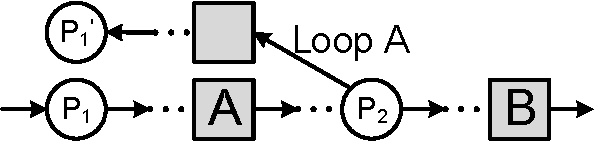
\includegraphics[width=1\textwidth]{causal_formula_a_1}
  	\end{minipage}
  	\begin{minipage}[b]{1\textwidth}
  	  \vspace{1em}
  	  \centering
  	  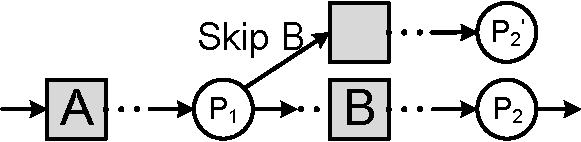
\includegraphics[width=1\textwidth]{causal_formula_a_2}
  	\end{minipage}
  	\caption{}
  	\label{fig:causal_formula_a}
  \end{subfigure}
  \begin{subfigure}{0.55\textwidth}
  	\centering
  	\begin{minipage}[b]{1\textwidth}
  	  \centering
  	  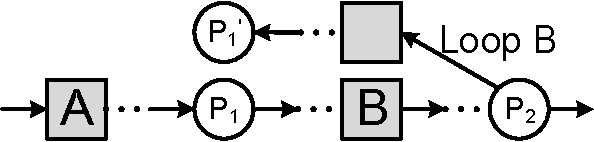
\includegraphics[width=1\textwidth]{causal_formula_b_1}
  	\end{minipage}
  	\begin{minipage}[b]{1\textwidth}
  	  \vspace{1em}
  	  \centering
  	  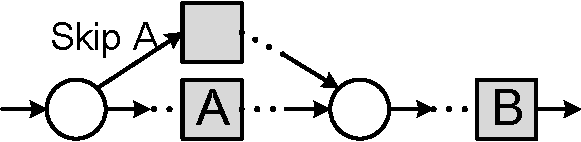
\includegraphics[width=1\textwidth]{causal_formula_b_2}
  	\end{minipage}
  	\caption{}
  	\label{fig:causal_formula_b}
  \end{subfigure}
  \begin{subfigure}{0.7\textwidth}
  	\vspace{1em}
  	\centering
  	\begin{minipage}[b]{1\textwidth}
  	  \centering
  	  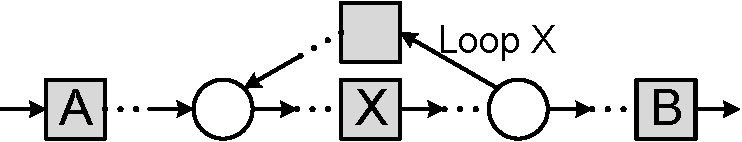
\includegraphics[width=1\textwidth]{causal_formula_c_1}
  	\end{minipage}
  	\begin{minipage}[b]{1\textwidth}
  	  \vspace{1em}
  	  \centering
  	  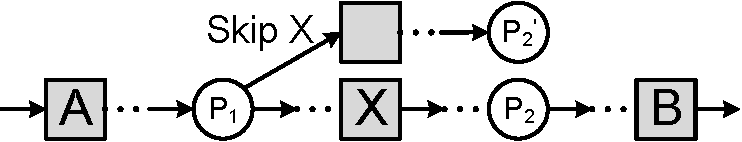
\includegraphics[width=1\textwidth]{causal_formula_c_2}
  	\end{minipage}
  	\caption{}
  	\label{fig:causal_formula_c}
  \end{subfigure}
  \begin{subfigure}{0.85\textwidth}
  	\vspace{1em}
  	\centering
  	\begin{minipage}[b]{1\textwidth}
  	  \centering
  	  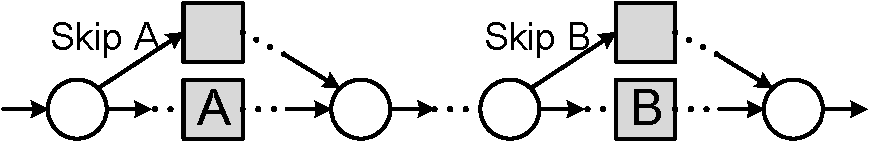
\includegraphics[width=1\textwidth]{causal_formula_d_1}
  	\end{minipage}
  	\begin{minipage}[b]{1\textwidth}
  	  \vspace{1em}
  	  \centering
  	  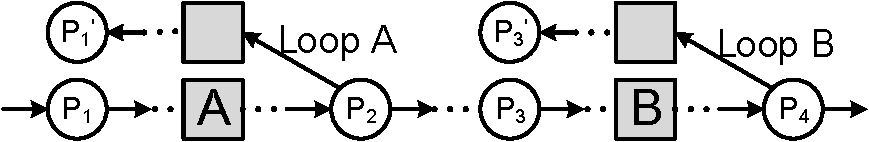
\includegraphics[width=1\textwidth]{causal_formula_d_2}
  	\end{minipage}
  	\caption{}
  	\label{fig:causal_formula_d}
  \end{subfigure}
  \caption{因果关系和逆因果关系的图形化抽象形式。\subref{fig:causal_formula_a} $A\overset{\text{\tiny{S}}}{\rightarrow}B$,$B\overset{\text{\tiny{A}}}{\leftarrow}A$;\subref{fig:causal_formula_b} $A\overset{\text{\tiny{A}}}{\rightarrow}B$,$B\overset{\text{\tiny{S}}}{\leftarrow}A$;\subref{fig:causal_formula_c} $A\overset{\text{\tiny{A}}}{\rightarrow}B$,$B\overset{\text{\tiny{A}}}{\leftarrow}A$;\subref{fig:causal_formula_d} $A\overset{\text{\tiny{S}}}{\rightarrow}B$,$B\overset{\text{\tiny{S}}}{\leftarrow}A$。}
  \label{fig:event_causal_formulas}
\end{figure}

图\ref{fig:causal_formula_a}中,上方的局部CPU有诸如$[A*B]$、$[A*A*B]$、$[A*A*A*B]$等形式的过程流,下方的局部CPU有诸如$[A*B]$、$[A*]$形式的过程流,根据定义\ref{def:exroru_event_causal}和定义\ref{def:exroru_event_inverse_causal},事件$A$和事件$B$满足“有时因果关系”和“总是逆因果关系”,即$A\overset{\text{\tiny{S}}}{\rightarrow}B$,$B\overset{\text{\tiny{A}}}{\leftarrow}A$;同理,\ref{fig:causal_formula_b}中,事件$A$和事件$B$满足“总是因果关系”和“有时逆因果关系”,即$A\overset{\text{\tiny{A}}}{\rightarrow}B$,$B\overset{\text{\tiny{S}}}{\leftarrow}A$。

图\ref{fig:causal_formula_c}中,局部CPU中间部分的循环结构和互斥结构显然不会影响事件$A$和事件$B$之间的因果关系和逆因果关系,两个局部CPU中的事件$A$和事件$B$都满足“总是因果关系”和“总是逆因果关系”,即$A\overset{\text{\tiny{A}}}{\rightarrow}B$,$B\overset{\text{\tiny{A}}}{\leftarrow}A$;然而,如果事件$A$和事件$B$都有与之相关的互斥结构,如图\ref{fig:causal_formula_d}上方局部CPU所示,其过程流有诸如$[A*B]$、$[A*]$、$[*B]$、$[*]$等形式,则事件$A$和事件$B$满足“有时因果关系”和“有时逆因果关系”,即$A\overset{\text{\tiny{S}}}{\rightarrow}B$,$B\overset{\text{\tiny{S}}}{\leftarrow}A$;同理,图\ref{fig:causal_formula_d}下方的局部CPU中事件$A$和事件$B$都有与之相关的循环结构,故事件$A$和事件$B$满足“有时因果关系”和“有时逆因果关系”,即$A\overset{\text{\tiny{S}}}{\rightarrow}B$,$B\overset{\text{\tiny{S}}}{\leftarrow}A$。

\subsection{事件间扩展不确定性精炼并行关系}\label{subsec:exroru_event_concurrent}
本文用形如$\langle abc\rangle$的表达式来描述轨迹。括号内的字母表示事件,其出现顺序和轨迹内对应事件的发生顺序相同。例如在图\ref{fig:case_study_cpu}的CPU中,$\langle I,A,C,D,O\rangle$、$\langle I,B,C,D,O\rangle$和$\langle I,D,E,D,A,C,O\rangle$都是一些轨迹示例。

令$\Omega_{x}$表示含有事件$x$的轨迹集合,即$\Omega_{x}=\{\sigma\in\Omega|x\in\sigma\}$。本文用$\sigma\uparrow X$表示轨迹$\sigma$到某些事件的集合$X\subseteq E$上的投影,即$\sigma$的子轨迹$\sigma'\subseteq\sigma$,其中$\sigma'$只含有集合$X$中的事件且其出现顺序保持和$\sigma$中一致。令$P(\sigma,x,y)=\sigma\uparrow\{x,y\}$表示轨迹$\sigma$到事件$x$和事件$y$上的投影。

\begin{definition}[事件间扩展不确定性精炼并行关系]\label{def:exroru_event_concurrent}
事件$x$和$y$满足:
  \begin{itemize}
  	\item[-] 总是并行关系(always concurrent relation),记作$x\Updownarrow y$,当且仅当:$\forall\sigma_{x}\in\Omega_{x}$,$x~co~y$且$P(\sigma,x,y)$满足正则表达式$[xy|yx|yy]*y?$\footnote{\url{https://en.wikipedia.org/wiki/Regular\_expression},正则表达式不是本文重点,对其详细的介绍可参见\onlinecite{mitkov2005oxford,lawson2003finite}}。
  	\item[-] 从不并行关系(never concurrent relation),记作$x\nparallel y$,当且仅当:$\forall\sigma_{x}\in\Omega_{x}$,$x$和$y$不满足定义\ref{def:ordering_relations}中的并行关系。
  	\item[-] 有时并行关系(sometimes concurrent relation),记作$x\Uparrow y$,当且仅当$x$和$y$不满足上述两种关系。
  \end{itemize}
\end{definition}

定义\ref{def:exroru_event_concurrent}中的关系统称扩展不确定性精炼并行关系(extended refined concurrent relations with uncertainty),用$\parallel$表示,本文在不引起歧义的情况下将其简称为并行关系。与因果关系和逆因果关系不同,ExRORU并不区分并行关系的直接并行关系和间接并行关系。

\begin{example}\label{ex:exroru_event_concurrent}
在图\ref{fig:case_study_cpu}的CPU中,事件$C$和事件$D$满足“总是并行关系”,即$C\Updownarrow D$,因为所有含有事件$C$的轨迹都满足定义\ref{def:exroru_event_concurrent}中的正则表达式;事件$D$和事件$C$满足“有时并行关系”,即$D\Uparrow C$,因为存在轨迹$\langle IDEDACO\rangle$,其在事件$D$和事件$C$上的投影为$\langle DDC\rangle$,该投影不满足定义\ref{def:exroru_event_concurrent}中的正则表达式;事件$I$和事件$O$满足“从不并行关系”,即$I\nparallel O$。
\end{example}

图\ref{fig:event_concurrent_formulas}给出了并行关系的图形化抽象形式。

\begin{figure}[htbp]
  \centering
  \begin{subfigure}{0.48\textwidth}
  	\centering
  	\begin{minipage}[b]{1\textwidth}
  	  \centering
  	  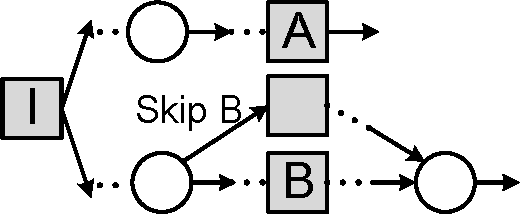
\includegraphics[width=1\textwidth]{concurrent_formula_a_1}
  	\end{minipage}
  	\begin{minipage}[b]{1\textwidth}
  	  \vspace{1em}
  	  \centering
  	  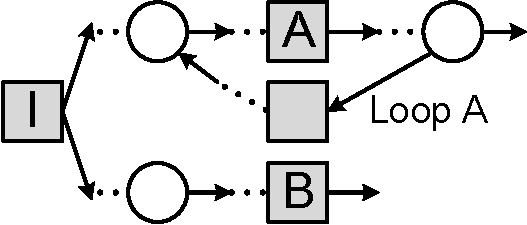
\includegraphics[width=1\textwidth]{concurrent_formula_a_2}
  	\end{minipage}
  	\caption{}
  	\label{fig:concurrent_formula_a}
  \end{subfigure}
  % \hspace{2em}
  \begin{subfigure}{0.48\textwidth}
  	\centering
  	\begin{minipage}[b]{1\textwidth}
  	  \centering
  	  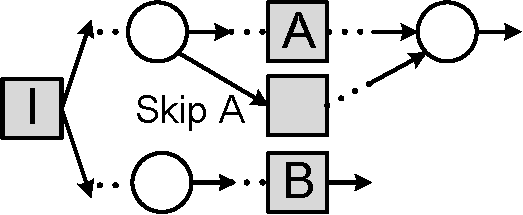
\includegraphics[width=1\textwidth]{concurrent_formula_b_1}
  	\end{minipage}
  	\begin{minipage}[b]{1\textwidth}
  	  \vspace{1em}
  	  \centering
  	  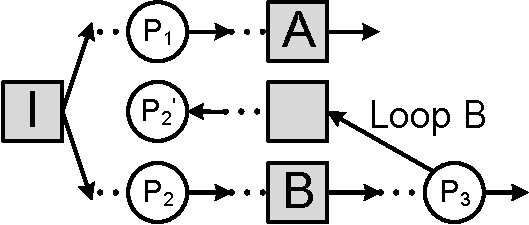
\includegraphics[width=1\textwidth]{concurrent_formula_b_2}
  	\end{minipage}
  	\caption{}
  	\label{fig:concurrent_formula_b}
  \end{subfigure}
  \begin{subfigure}{0.48\textwidth}
  	\vspace{1em}
  	\centering
  	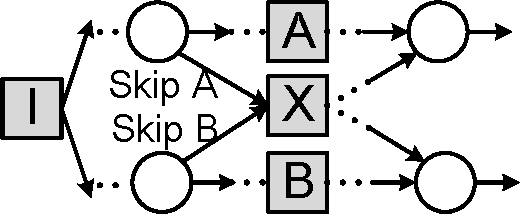
\includegraphics[width=1\textwidth]{concurrent_formula_c}
  	\caption{}
  	\label{fig:concurrent_formula_c}
  \end{subfigure}
  \begin{subfigure}{0.48\textwidth}
  	\vspace{1em}
  	\centering
  	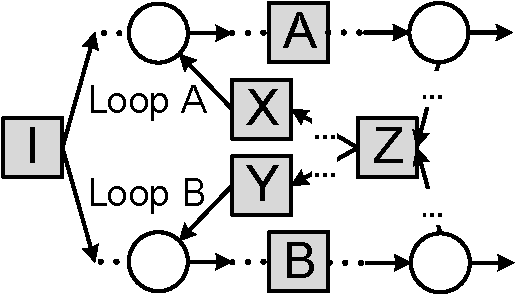
\includegraphics[width=1\textwidth]{concurrent_formula_d}
  	\caption{}
  	\label{fig:concurrent_formula_d}
  \end{subfigure}
  \begin{subfigure}{0.48\textwidth}
  	\vspace{1em}
  	\centering
  	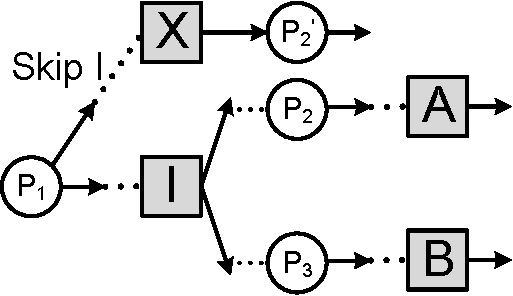
\includegraphics[width=1\textwidth]{concurrent_formula_e}
  	\caption{}
  	\label{fig:concurrent_formula_e}
  \end{subfigure}
  \caption{并行关系的图形化抽象形式。\subref{fig:concurrent_formula_a} $A\Uparrow B$,$B\Updownarrow A$;\subref{fig:concurrent_formula_b} $A\Updownarrow B$,$B\Uparrow A$;\subref{fig:concurrent_formula_c} $A\Updownarrow B$,$B\Updownarrow A$;\subref{fig:concurrent_formula_d} $A\Updownarrow B$,$B\Updownarrow A$;\subref{fig:concurrent_formula_e} $A\Uparrow B$,$B\Updownarrow A$。}
  \label{fig:event_concurrent_formulas}
\end{figure}

图\ref{fig:concurrent_formula_a}中,上方的局部CPU有诸如$\langle I*A*B*\rangle$、$\langle I*B*A*\rangle$、$\langle I*A*\rangle$等形式的轨迹,下方的局部CPU有诸如$\langle I*A*B*\rangle$、$\langle I*A*A*B*\rangle$、$\langle I*A*A*A*B*\rangle$等形式的轨迹。当考察事件$A$和事件$B$的并行关系时,轨迹不符合定义\ref{def:exroru_event_concurrent}中的正则表达式,因此事件$A$和事件$B$满足“有时并行关系”,即$A\Uparrow B$;然而,当考察事件$B$和事件$A$的并行关系时,轨迹符合定义\ref{def:exroru_event_concurrent}中的正则表达式,因此事件$B$和事件$A$满足“总是并行关系”,即$B\Updownarrow A$。

图\ref{fig:concurrent_formula_b}中,上方的局部CPU有诸如$\langle I*A*B*\rangle$、$\langle I*B*A*\rangle$、$\langle I*B*\rangle$等形式的轨迹,下方的局部CPU有诸如$\langle I*A*B*\rangle$、$\langle I*A*B*B*\rangle$、$\langle I*A*B*B*B*\rangle$等形式的轨迹。当考察事件$A$和事件$B$的并行关系时,轨迹符合定义\ref{def:exroru_event_concurrent}中的正则表达式,因此事件$A$和事件$B$满足“总是并行关系”,即$A\Updownarrow B$;然而,当考察事件$B$和事件$A$的并行关系时,轨迹不符合定义\ref{def:exroru_event_concurrent}中的正则表达式,因此事件$B$和事件$A$满足“有时并行关系”,即$B\Uparrow A$。

图\ref{fig:concurrent_formula_c}中的局部CPU有诸如$\langle I*A*B*\rangle$、$\langle I*B*A*\rangle$、$\langle I*X*\rangle$等形式的轨迹,事件$A$和事件$B$要么都被执行一次,要么都不被执行,因此事件$A$和事件$B$满足“总是并行关系”,即$A\Updownarrow B$,反之亦然,即$B\Updownarrow A$。类似的,在图\ref{fig:concurrent_formula_d}中的局部CPU中,事件$A$和事件$B$要么都被执行一次,要么都被执行两次……以此类推,它们被执行的次数相同且与循环次数有关。显然,含有事件$A$或者$B$的轨迹都符合定义\ref{def:exroru_event_concurrent}中的正则表达式,因此事件$A$和事件$B$满足“总是并行关系”,即$A\Updownarrow B$,反之亦然,即$B\Updownarrow A$。

图\ref{fig:concurrent_formula_d}中的局部CPU展示了一个非自由选择结构的部分,其有诸如$\langle *I*A*B*\rangle$、$\langle *I*B*A*\rangle$、$\langle *X*A*\rangle$等形式的轨迹。当考察事件$A$和事件$B$的并行关系时,含有事件$A$的轨迹不一定包含事件$B$,故事件$A$和事件$B$满足“有时并行关系”,即$A\Uparrow B$;当考察事件$B$和事件$A$的并行关系时,含有事件$B$的轨迹一定包含事件$A$,且轨迹符合定义\ref{def:exroru_event_concurrent}中的正则表达式,故事件$B$和事件$A$满足“总是并行关系”,即$B\Updownarrow A$。本文将会对非自由选择结构进行更为详细的探讨。

表\ref{tab:exroru_event}给出了所有的事件间ExRORU关系,共11种。

\begin{table}[htbp]
  \centering
  \begin{minipage}[t]{0.8\textwidth}
  	\caption{事件间ExRORU关系概览}
  	\label{tab:exroru_event}
  	\begin{tabularx}{\textwidth}{clclcl}
  	  \toprule[1.5pt]
  	  关系 & 描述 & 关系 & 描述 & 关系 & 描述 \\\midrule[1pt]
  	  $\overset{\text{\tiny{DA}}}{\rightarrow}$ & 直接总是因果 & $\overset{\text{\tiny{DA}}}{\leftarrow}$ & 直接总是逆因果 & $\Updownarrow$ & 总是并行\\
  	  $\overset{\text{\tiny{IA}}}{\rightarrow}$ & 间接总是因果 & $\overset{\text{\tiny{IA}}}{\leftarrow}$ & 间接总是逆因果 & $\Uparrow$ & 有时并行\\
  	  $\overset{\text{\tiny{DS}}}{\rightarrow}$ & 直接有时因果 & $\overset{\text{\tiny{DS}}}{\leftarrow}$ & 直接有时逆因果 & $\nparallel$ & 从不并行\\
  	  $\overset{\text{\tiny{IS}}}{\rightarrow}$ & 间接有时因果 & $\overset{\text{\tiny{IS}}}{\leftarrow}$ & 间接有时逆因果 & & \\
  	  $\overset{\text{\tiny{N}}}{\rightarrow}$ & 从不因果 & $\overset{\text{\tiny{N}}}{\leftarrow}$ & 从不逆因果 & & \\
  	  \bottomrule[1.5pt]
  	\end{tabularx}
  \end{minipage}
\end{table}

\begin{example}\label{ex:case_study_exroru_event_matrix}
表\ref{tab:case_study_exroru_event_matrix}展示了图\ref{fig:case_study_cpu}中CPU的事件间ExRORU关系。三个矩阵分别对应因果关系、逆因果关系和并行关系。每个单元格内显示了该单元格所对应的行列对$(X,Y)$之间的ExRORU关系。
\end{example}

\begin{table}[htbp]
  \centering
  \caption{图\ref{fig:case_study_cpu}中CPU的事件间ExRORU关系}
  \label{tab:case_study_exroru_event_matrix}
  \begin{subtable}{0.45\textwidth}
    \centering
    \caption{因果关系(5种)}
    \begin{tabular}{|c|c|c|c|c|c|c|c|} \hline
	  $\rightarrow$ & $A$ & $B$ & $C$ & $D$ & $E$ & $I$ & $O$\\ \hline
	  $A$ & $\overset{\text{\tiny{N}}}{\rightarrow}$ & $\overset{\text{\tiny{N}}}{\rightarrow}$ & $\overset{\text{\tiny{DA}}}{\rightarrow}$ & $\overset{\text{\tiny{N}}}{\rightarrow}$ & $\overset{\text{\tiny{N}}}{\rightarrow}$ & $\overset{\text{\tiny{N}}}{\rightarrow}$ & $\overset{\text{\tiny{IA}}}{\rightarrow}$\\ \hline
	  $B$ & $\overset{\text{\tiny{N}}}{\rightarrow}$ & $\overset{\text{\tiny{N}}}{\rightarrow}$ & $\overset{\text{\tiny{DA}}}{\rightarrow}$ & $\overset{\text{\tiny{N}}}{\rightarrow}$ & $\overset{\text{\tiny{N}}}{\rightarrow}$ & $\overset{\text{\tiny{N}}}{\rightarrow}$ & $\overset{\text{\tiny{IA}}}{\rightarrow}$\\ \hline
	  $C$ & $\overset{\text{\tiny{N}}}{\rightarrow}$ & $\overset{\text{\tiny{N}}}{\rightarrow}$ & $\overset{\text{\tiny{N}}}{\rightarrow}$ & $\overset{\text{\tiny{N}}}{\rightarrow}$ & $\overset{\text{\tiny{N}}}{\rightarrow}$ & $\overset{\text{\tiny{N}}}{\rightarrow}$ & $\overset{\text{\tiny{DA}}}{\rightarrow}$\\ \hline
	  $D$ & $\overset{\text{\tiny{N}}}{\rightarrow}$ & $\overset{\text{\tiny{N}}}{\rightarrow}$ & $\overset{\text{\tiny{N}}}{\rightarrow}$ & $\overset{\text{\tiny{IS}}}{\rightarrow}$ & $\overset{\text{\tiny{DS}}}{\rightarrow}$ & $\overset{\text{\tiny{N}}}{\rightarrow}$ & $\overset{\text{\tiny{DS}}}{\rightarrow}$\\ \hline
	  $E$ & $\overset{\text{\tiny{N}}}{\rightarrow}$ & $\overset{\text{\tiny{N}}}{\rightarrow}$ & $\overset{\text{\tiny{N}}}{\rightarrow}$ & $\overset{\text{\tiny{DA}}}{\rightarrow}$ & $\overset{\text{\tiny{IS}}}{\rightarrow}$ & $\overset{\text{\tiny{N}}}{\rightarrow}$ & $\overset{\text{\tiny{IA}}}{\rightarrow}$\\ \hline
	  $I$ & $\overset{\text{\tiny{DS}}}{\rightarrow}$ & $\overset{\text{\tiny{DS}}}{\rightarrow}$ & $\overset{\text{\tiny{IA}}}{\rightarrow}$ & $\overset{\text{\tiny{DA}}}{\rightarrow}$ & $\overset{\text{\tiny{IS}}}{\rightarrow}$ & $\overset{\text{\tiny{N}}}{\rightarrow}$ & $\overset{\text{\tiny{IA}}}{\rightarrow}$\\ \hline
	  $O$ & $\overset{\text{\tiny{N}}}{\rightarrow}$ & $\overset{\text{\tiny{N}}}{\rightarrow}$ & $\overset{\text{\tiny{N}}}{\rightarrow}$ & $\overset{\text{\tiny{N}}}{\rightarrow}$ & $\overset{\text{\tiny{N}}}{\rightarrow}$ & $\overset{\text{\tiny{N}}}{\rightarrow}$ & $\overset{\text{\tiny{N}}}{\rightarrow}$\\ \hline
	\end{tabular}
  \end{subtable}
  \hspace{1em}
  \begin{subtable}{0.45\textwidth}
    \centering
    \caption{逆因果关系(5种)}
	\begin{tabular}{|c|c|c|c|c|c|c|c|} \hline
		$\leftarrow$ & $A$ & $B$ & $C$ & $D$ & $E$ & $I$ & $O$\\ \hline
		$A$ & $\overset{\text{\tiny{N}}}{\leftarrow}$ & $\overset{\text{\tiny{N}}}{\leftarrow}$ & $\overset{\text{\tiny{N}}}{\leftarrow}$ & $\overset{\text{\tiny{N}}}{\leftarrow}$ & $\overset{\text{\tiny{N}}}{\leftarrow}$ & $\overset{\text{\tiny{DA}}}{\leftarrow}$ & $\overset{\text{\tiny{N}}}{\leftarrow}$\\ \hline
		$B$ & $\overset{\text{\tiny{N}}}{\leftarrow}$ & $\overset{\text{\tiny{N}}}{\leftarrow}$ & $\overset{\text{\tiny{N}}}{\leftarrow}$ & $\overset{\text{\tiny{N}}}{\leftarrow}$ & $\overset{\text{\tiny{N}}}{\leftarrow}$ & $\overset{\text{\tiny{DA}}}{\leftarrow}$ & $\overset{\text{\tiny{N}}}{\leftarrow}$\\ \hline
		$C$ & $\overset{\text{\tiny{DS}}}{\leftarrow}$ & $\overset{\text{\tiny{DS}}}{\leftarrow}$ & $\overset{\text{\tiny{N}}}{\leftarrow}$ & $\overset{\text{\tiny{N}}}{\leftarrow}$ & $\overset{\text{\tiny{N}}}{\leftarrow}$ & $\overset{\text{\tiny{IA}}}{\leftarrow}$ & $\overset{\text{\tiny{N}}}{\leftarrow}$\\ \hline
		$D$ & $\overset{\text{\tiny{N}}}{\leftarrow}$ & $\overset{\text{\tiny{N}}}{\leftarrow}$ & $\overset{\text{\tiny{N}}}{\leftarrow}$ & $\overset{\text{\tiny{IS}}}{\leftarrow}$ & $\overset{\text{\tiny{DS}}}{\leftarrow}$ & $\overset{\text{\tiny{DS}}}{\leftarrow}$ & $\overset{\text{\tiny{N}}}{\leftarrow}$\\ \hline
		$E$ & $\overset{\text{\tiny{N}}}{\leftarrow}$ & $\overset{\text{\tiny{N}}}{\leftarrow}$ & $\overset{\text{\tiny{N}}}{\leftarrow}$ & $\overset{\text{\tiny{DA}}}{\leftarrow}$ & $\overset{\text{\tiny{IS}}}{\leftarrow}$ & $\overset{\text{\tiny{IS}}}{\leftarrow}$ & $\overset{\text{\tiny{N}}}{\leftarrow}$\\ \hline
		$I$ & $\overset{\text{\tiny{N}}}{\leftarrow}$ & $\overset{\text{\tiny{N}}}{\leftarrow}$ & $\overset{\text{\tiny{N}}}{\leftarrow}$ & $\overset{\text{\tiny{N}}}{\leftarrow}$ & $\overset{\text{\tiny{N}}}{\leftarrow}$ & $\overset{\text{\tiny{N}}}{\leftarrow}$ & $\overset{\text{\tiny{N}}}{\leftarrow}$\\ \hline
		$O$ & $\overset{\text{\tiny{IS}}}{\leftarrow}$ & $\overset{\text{\tiny{IS}}}{\leftarrow}$ & $\overset{\text{\tiny{DA}}}{\leftarrow}$ & $\overset{\text{\tiny{DA}}}{\leftarrow}$ & $\overset{\text{\tiny{IS}}}{\leftarrow}$ & $\overset{\text{\tiny{IA}}}{\leftarrow}$ & $\overset{\text{\tiny{N}}}{\leftarrow}$\\ \hline
	\end{tabular}
  \end{subtable}
  \begin{subtable}{\textwidth}
  	\vspace{1em}
    \centering
    \caption{并行关系(3种)}
	\begin{tabular}{|c|c|c|c|c|c|c|c|} \hline
		$\parallel$ & $A$ & $B$ & $C$ & $D$ & $E$ & $I$ & $O$\\ \hline
		$A$ & $\nparallel$ & $\nparallel$ & $\nparallel$ & $\Updownarrow$ & $\Uparrow$ & $\nparallel$ & $\nparallel$\\ \hline
		$B$ & $\nparallel$ & $\nparallel$ & $\nparallel$ & $\Updownarrow$ & $\Uparrow$ & $\nparallel$ & $\nparallel$\\ \hline
		$C$ & $\nparallel$ & $\nparallel$ & $\nparallel$ & $\Updownarrow$ & $\Uparrow$ & $\nparallel$ & $\nparallel$\\ \hline
		$D$ & $\Uparrow$ & $\Uparrow$ & $\Uparrow$ & $\nparallel$ & $\nparallel$ & $\nparallel$ & $\nparallel$\\ \hline
		$E$ & $\Uparrow$ & $\Uparrow$ & $\Uparrow$ & $\nparallel$ & $\nparallel$ & $\nparallel$ & $\nparallel$\\ \hline
		$I$ & $\nparallel$ & $\nparallel$ & $\nparallel$ & $\nparallel$ & $\nparallel$ & $\nparallel$ & $\nparallel$\\ \hline
		$O$ & $\nparallel$ & $\nparallel$ & $\nparallel$ & $\nparallel$ & $\nparallel$ & $\nparallel$ & $\nparallel$\\ \hline
	\end{tabular}
  \end{subtable}
\end{table}

\subsection{基于CPU计算事件间ExRORU关系}\label{subsec:exroru_event_computation}
一个直观方法是直接依据定义\ref{def:exroru_event_causal}、\ref{def:exroru_event_inverse_causal}、\ref{def:exroru_event_concurrent}计算事件间ExRORU关系,然而由于循环结构的存在,一个CPU可能有无穷多个过程流和轨迹,无法应用上述定义计算关系。另一方面,在一个含有多并发分支结构的CPU中,计算其轨迹集合会导致状态爆炸问题。因此,直接利用过程流和轨迹计算ExRORU关系是不合适的,本文使用定义\ref{def:cpu}中提出的完全前缀展开计算事件间ExRORU关系。

在计算事件$A$和事件$B$之间的因果关系时,可以借助图\ref{fig:event_causal_formulas}中的因果关系抽象形式,从CPU中抽取一条从$A$到$B$的路径,并依次遍历其中的条件以判断是否存在符合抽象形式中的“Skip”或者“Loop”结构,从而得到事件$A$和事件$B$之间的因果关系。

算法\ref{algo:exroru_event_causal}给出了计算事件间因果关系的伪代码。算法接收完全前缀展开$U$和两个事件$A$、$B$作为输入,输出事件$A$和事件$B$之间的因果关系。算法分两种情况抽取因果关系:若事件$A$和事件$B$是相同事件(第1行),则尝试在$U$中找一条从事件$A$到自身的自循环路径,若该路径存在说明事件$A$与自身满足“有时因果关系”(第2-3行),否则满足“从不因果关系”(第4-5行);若事件$A$和事件$B$是不同事件(第6行),则尝试在$U$中找一条从事件$A$到事件$B$的路径,若该路径存在(第7行),则依次遍历路径上的XOR-split条件并寻找图\ref{fig:event_causal_formulas}中的“Loop”和“Skip”结构(第8-9行),若该类结构存在说明事件$A$和事件$B$满足“有时因果关系”(第10行),否则说明事件$A$和事件$B$满足“总是因果关系”(第11行),若从$A$到$B$的路径不存在,说明事件$A$和事件$B$满足“从不因果关系”(第12-13行)。

\begin{algorithm}[htbp]
  \LinesNumbered
  \caption{计算事件间因果关系}
  \label{algo:exroru_event_causal}
  \KwIn{完全前缀展开$U$,事件$A$和事件$B$}
  \KwOut{事件$A$和事件$B$之间的因果关系}
  \uIf{$A=B$} {
  	\uIf{\textnormal{There exists a path from $A$ to $B$}} {
  	  \Return{$A\overset{\text{\tiny{S}}}{\rightarrow}B$}
  	} \Else {
  	  \Return{$A\overset{\text{\tiny{N}}}{\rightarrow}B$}
  	}
  } \Else {
  	\uIf{\textnormal{There exists a path $s$ from $A$ to $B$}} {
  	  \For{\textnormal{XOR-split condition $X$ in $s$}} {
  	  	\If{\textnormal{There exists another path from $X$ to $A$ (``loop $A$'') or from $X$ to sink condition without $B$ (``skip $B$'')}} {
  	  	  \Return{$A\overset{\text{\tiny{S}}}{\rightarrow}B$}
  	  	}
  	  }
  	  \Return{$A\overset{\text{\tiny{A}}}{\rightarrow}B$}
  	} \Else {
  	  \Return{$A\overset{\text{\tiny{N}}}{\rightarrow}B$}
  	}
  }
\end{algorithm}

\textcolor{red}{证明任意一条路径都能抽取正确的关系}

类似的,在计算事件$B$和事件$A$的逆因果关系时,同样可以借助图\ref{fig:event_causal_formulas}中的因果关系抽象形式,从CPU中抽取一条从$A$到$B$的路径,并逆向遍历其中的条件以判断是否存在符合抽象形式中的“Skip”或者“Loop”结构,从而得到事件$B$和事件$A$之间的逆因果关系。与算法\ref{algo:exroru_event_causal}不同的是,在计算事件$B$和事件$A$的逆因果关系时,需要关注的是路径中的XOR-join条件而不是XOR-split条件。

\textcolor{red}{计算直接因果关系的算法}

需要注意的是,对于一对事件$A$和$B$,其因果关系$A\rightarrow B$和逆因果关系$B\leftarrow A$可能有着不同的不确定性。例如,在图\ref{fig:case_study_cpu}所示的CPU中,事件$A$和事件$O$满足“间接总是因果关系”,即$A\overset{\text{\tiny{IA}}}{\rightarrow}O$;而事件$O$和事件$A$满足“间接有时逆因果关系”,即$O\overset{\text{\tiny{IS}}}{\leftarrow}A$。另外,事件$D$和事件$E$满足“直接有时因果关系”,即$D\overset{\text{\tiny{DS}}}{\rightarrow}E$;而事件$E$和事件$D$满足“直接总是逆因果关系”,即$E\overset{\text{\tiny{DA}}}{\leftarrow}D$。由于循环结构的存在,事件$D$和事件$E$之间的因果关系不能被RORU算法正确识别。

在计算事件$A$和事件$B$之间的并行关系时,实际上需要考虑两个方向并行关系的不确定性,即$A\parallel B$和$B\parallel A$。类似的,可以借助图\ref{fig:event_concurrent_formulas}中的并行关系抽象形式,首先找到两个事件的并行结构入口,并依次遍历从入口分别到事件$A$、事件$B$的路径以判断是否存在符合抽象形式中的“Skip”或者“Loop”结构,从而得到事件$A$和事件$B$之间的并行关系。

算法\ref{algo:exroru_event_concurrent}给出了计算事件间并行关系的伪代码。算法接收完全前缀展开$U$和两个事件$A$、$B$作为输入,输出事件$A$和事件$B$之间的双向并行关系。算法首先判断事件$A$和事件$B$是否满足并行关系(第1行):若不满足,则事件$A$和事件$B$满足“从不并行关系”,即$A\nparallel B$,且事件$B$和事件$A$也满足“从不并行关系”,即$B\nparallel A$(第2行);否则,分别寻找从并行结构入口到事件$A$的路径$s_{1}$和从并行结构入口到事件$B$的路径$s_{2}$(第3-5行),然后依次检查$s_{1}$和$s_{2}$上的XOR-split和XOR-join条件节点(第6-7行),并依据上述检查结果判定事件$A$和事件$B$的并行关系不确定性(第8-9行)。

\begin{algorithm}[htbp]
  \LinesNumbered
  \caption{计算事件间并行关系}
  \label{algo:exroru_event_concurrent}
  \SetKwFunction{xorsplitfunc}{CheckXORSplit}
  \SetKwFunction{xorjoinfunc}{CheckXORJoin}
  \KwIn{完全有限前缀$U$,事件$A$和事件$B$}
  \KwOut{事件$A$和事件$B$之间的并行关系}
  \uIf{\textnormal{$A=B~or$ they are not in concurrent relation}} {
  	\Return{$A\nparallel B,B\nparallel A$}
  } \Else {
  	Mark the concurrent entrance as $lcp(A,B)$ or $lcp$\;
  	Find the path $s_{1}$ from $lcp$ to $A$ and the path $s_{2}$ from $lcp$ to $B$\;
  	$(A\&B)_{1},(B\&A)_{1}\leftarrow\xorsplitfunc{$lcp,A,B,s_{1},s_{2}$}$\;
  	$(A\&B)_{2},(B\&A)_{2}\leftarrow\xorjoinfunc{$lcp,A,B,s_{1},s_{2}$}$\;
  	\Return{$(A\&B)_{1}=\text{``Always''}\wedge(A\&B)_{2}=\text{``Always''}~?~A\Updownarrow B~:~A\Uparrow B,$\\\qquad\quad$(B\&A)_{1}=\text{``Always''}\wedge(B\&A)_{2}=\text{``Always''}~?~B\Updownarrow A~:~B\Uparrow A$}
  }
\end{algorithm}

算法\ref{algo:exroru_event_concurrent}中对于XOR-split节点的处理(第6行)如算法\ref{algo:exroru_event_concurrent_xorsplit}所示。函数\texttt{CheckXORSplit}接收并行结构入口$lcp$、事件$A$、事件$B$和从并行结构入口到事件$A$和$B$的路径$s_{1}$和$s_{2}$作为参数,返回两条路径XOR-split节点作用下的事件$A$和事件$B$之间的双向并行关系。函数首先初始化双向并行关系不确定性为“Always”(第1行),然后遍历两条路径找到所有满足抽象形式的XOR-split节点(第2-3行)。接下来,函数执行两重循环处理未被访问过的XOR-split节点(第4-5行),若满足图\ref{fig:concurrent_formula_c}的抽象形式($lcs(a_{i},b_{j})$表示两个节点的最近公共后继,即抽象形式中的变迁$X$),则将这两个节点标记为“已访问”(第6-7行);否则事件$A$和事件$B$满足“有时并行关系”,即$A\Uparrow B$,且事件$B$和事件$A$也满足“有时并行关系”,即$B\Uparrow A$(第8-9行)。最后函数依据未访问过的XOR-split节点返回XOR-split作用下的事件$A$和事件$B$之间的双向并行关系(第10-14行)。

\begin{algorithm}[htbp]
  \LinesNumbered
  \caption{检查XOR-split节点}
  \label{algo:exroru_event_concurrent_xorsplit}
  \SetKwProg{Fn}{Function}{}{}
  \Fn{\xorsplitfunc{$lcp,A,B,s_{1},s_{2}$}} {
  	\nl $A\&B\leftarrow\text{``Always''},B\&A\leftarrow\text{``Always''}$\;
  	\nl Assume there are XOR-splits $a_{1},a_{2},...,a_{m}$ which ``skips $A$'' in $s_{1}$\;
  	\nl Assume there are XOR-splits $b_{1},b_{2},...,b_{n}$ which ``skips $B$'' in $s_{2}$\;
  	\nl \For{$i=1$ \KwTo $m$\textnormal{ and $a_{i}$ is not marked as ``visited''}} {
  	  \nl \For{$j=1$ \KwTo $n$\textnormal{ and $b_{j}$ is not marked as ``visited''}} {
  	    \nl \uIf{\textnormal{$lcs(a_{i},b_{j})$ is an event and $a_{i}\nrightarrow lcs(a_{i},b_{j})\wedge b_{j}\nrightarrow lcs(a_{i},b_{j})$}} {
  	      \nl Mark $a_{i}$ and $b_{j}$ as ``visited''\;
  	    } \nl \Else {
  	      \nl \Return{$A\&B\leftarrow\text{``Sometimes''},B\&A\leftarrow\text{``Sometimes''}$}
  	    }
  	  }
  	}
  	\nl \If{\textnormal{There exists $1\leq i\leq m$ such that $a_{i}$ is not marked ``visited''}} {
  	  \nl $B\&A\leftarrow\text{``Sometimes''}$\;
  	}
  	\nl \If{\textnormal{There exists $1\leq j\leq n$ such that $b_{j}$ is not marked ``visited''}} {
  	  \nl $A\&B\leftarrow\text{``Sometimes''}$\;
  	}
  	\nl \Return{$A\&B,B\&A$}
  }
\end{algorithm}

算法\ref{algo:exroru_event_concurrent}中对于XOR-join节点的处理(第7行)如算法\ref{algo:exroru_event_concurrent_xorjoin}所示。函数\texttt{CheckXORJoin}接收并行结构入口$lcp$、事件$A$、事件$B$和从并行结构入口到事件$A$和事件$B$的路径$s_{1}$和$s_{2}$作为参数,返回两条路径XOR-join节点作用下的事件$A$和事件$B$之间的双向并行关系。函数首先初始化双向并行关系不确定性为“Always”(第1行),然后遍历两条路径找到所有满足抽象形式的XOR-join节点(第2-3行)。接下来,函数执行两重循环处理未被访问过的XOR-join节点(第4-5行),若满足图\ref{fig:concurrent_formula_d}的抽象形式($lcp(a_{i},b_{j})$表示两个节点的最近公共前驱,即抽象形式中的变迁$X$),则将这两个节点标记为“已访问”(第6-7行);否则事件$A$和事件$B$满足“有时并行关系”,即$A\Uparrow B$,且事件$B$和事件$A$也满足“有时并行关系”,即$B\Uparrow A$(第8-9行)。最后函数依据未访问过的XOR-join节点返回XOR-join作用下的事件$A$和事件$B$之间的双向并行关系(第10-14行)。

\begin{algorithm}[htbp]
  \LinesNumbered
  \caption{检查XOR-join节点}
  \label{algo:exroru_event_concurrent_xorjoin}
  \SetKwProg{Fn}{Function}{}{}
  \Fn{\xorjoinfunc{$lcp,A,B,s_{1},s_{2}$}} {
    \nl $A\&B\leftarrow\text{``Always''},B\&A\leftarrow\text{``Always''}$\;
    \nl Assume there are XOR-joins $a_{1},a_{2},...,a_{m}$ which ``skips $lcp$'' or ``loops $A$''\;
    \nl Assume there are XOR-joins $b_{1},b_{2},...,b_{n}$ which ``skips $lcp$'' or ``loops $B$''\;
    \nl \For{$i=1$ \KwTo $m$\textnormal{ and $a_{i}$ is not marked as ``visited''}} {
      \nl \For{$j=1$ \KwTo $n$\textnormal{ and $b_{j}$ is not marked as ``visited''}} {
        \nl \uIf{\textnormal{$lcp(a_{i},b_{j})$ is a condition or $lcp(a_{i},b_{j})=lcp$}} {
  	      \nl \Return{$A\&B\leftarrow\text{``Sometimes''},B\&A\leftarrow\text{``Sometimes''}$}
        } \nl \Else {
          \nl Mark $a_{i}$ and $b_{j}$ as ``visited''\;
        }
      }
    }
    \nl \If{\textnormal{There exists $1\leq i\leq m$ such that $a_{i}$ is not marked ``visited''}} {
  	  \nl $B\&A\leftarrow\text{``Sometimes''}$\;
  	}
  	\nl \If{\textnormal{There exists $1\leq j\leq n$ such that $b_{j}$ is not marked ``visited''}} {
  	  \nl $A\&B\leftarrow\text{``Sometimes''}$\;
  	}
  	\nl \Return{$A\&B,B\&A$}
  }
\end{algorithm}

\section{变迁间扩展不确定性精炼有序关系}\label{sec:exroru_transition}
本小节重点介绍如何折叠定义\ref{def:exroru_event_causal}、定义\ref{def:exroru_event_inverse_causal}和定义\ref{def:exroru_event_concurrent}中的事件间ExRORU关系得到原WF-net中变迁间ExRORU关系。一个WF-net中的变迁可能对应其CPU中的多个事件。这些对应的事件互不相同,在获取CPU中事件间ExRORU关系时都被当作独立事件处理。然而,这多个对应的事件与其他事件间的ExRORU关系通常是不一样的。因此,在获取WF-net中变迁间ExRORU关系时,需要逐一检查这些对应事件与其他变迁的对应事件间的关系,并将不同的事件间ExRORU关系折叠得到变迁间ExRORU关系。

上述情况出现的一个典型场景是含有非自由选择结构的过程模型。图\ref{fig:nfc_exroru}展示了一个含有非自由选择结构的WF-net及其对应的CPU。图\ref{fig:nfc_petri}所示WF-net中的变迁$C$对应了图\ref{fig:nfc_cpu}所示CPU中的事件$C_{1}$和事件$C_{2}$。根据定义\ref{def:exroru_event_causal},事件$C_{1}$和事件$D$满足“直接总是因果关系”而事件$C_{2}$和事件$D$满足“从不因果关系”,即$C_{1}\overset{\text{\tiny{DA}}}{\rightarrow}D$,$C_{2}\overset{\text{\tiny{N}}}{\rightarrow}D$。

\begin{figure}[htbp]
  \centering
  \begin{subfigure}{1\textwidth}
    \centering
    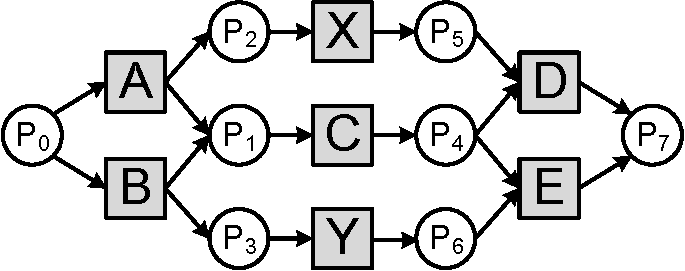
\includegraphics[width=0.7\textwidth]{nfc_petri}
    \caption{含有非自由选择结构的WF-net}
    \label{fig:nfc_petri}
  \end{subfigure}
  \begin{subfigure}{1\textwidth}
    \vspace{1em}
    \centering
    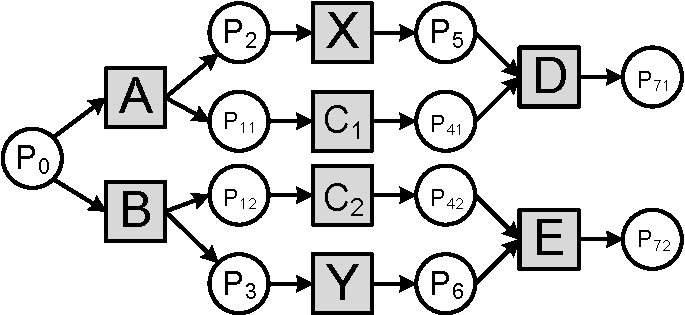
\includegraphics[width=0.7\textwidth]{nfc_cpu}
    \caption{图\subref{fig:nfc_petri}中WF-net对应的CPU}
    \label{fig:nfc_cpu}
  \end{subfigure}
  \caption{RORU无法区分的一对含有不可见变迁的模型}
  \label{fig:nfc_exroru}
\end{figure}

\subsection{变迁间扩展不确定性精炼有序关系的定义}\label{subsec:exroru_transition_def}
定义\ref{def:exroru_transition_causal}、\ref{def:exroru_transition_inverse_causal}、\ref{def:exroru_transition_concurrent}定性给出了上述折叠过程。令$\Sigma=(P,T,F,M_{0})$是一个WF-net,$U=(B,E,A,f)$是其CPU,$A,B\in T$是$\Sigma$的两个变迁。用$map$-$to$-$events(A)$表示变迁$A$在CPU中对应的所有事件集合。

\begin{definition}[变迁间扩展不确定性精炼因果关系]\label{def:exroru_transition_causal}
变迁$A$和$B$满足:
  \begin{itemize}
    \item[-] 总是因果关系(always causal relation),记作$A\overset{\text{\tiny{A}}}{\rightarrow}B$,当且仅当:$\forall a\in map$-$to$-$events(A),\exists b\in map$-$to$-$events(B),s.t.~a\overset{\text{\tiny{A}}}{\rightarrow}b$。
    \item[-] 从不因果关系(never causal relation),记作$A\overset{\text{\tiny{N}}}{\rightarrow}B$,当且仅当:$\forall a\in map$-$to$-$events(A),\forall b\in map$-$to$-$events(B),s.t.~a\overset{\text{\tiny{N}}}{\rightarrow}b$。
    \item[-] 有时因果关系(sometimes causal relation),记作$A\overset{\text{\tiny{S}}}{\rightarrow}B$,当且仅当$A$和$B$不满足上述两种关系。
  \end{itemize}
进一步,如果$\exists a\in map$-$to$-$events(A),\exists b\in map$-$to$-$events(B),s.t.~a\overset{\text{\tiny{DA}}}{\rightarrow}b$或者$a\overset{\text{\tiny{DS}}}{\rightarrow}b$,则$A\overset{\text{\tiny{DA}}}{\rightarrow}B$或者$A\overset{\text{\tiny{DS}}}{\rightarrow}B$;否则$A\overset{\text{\tiny{IA}}}{\rightarrow}B$或者$A\overset{\text{\tiny{IS}}}{\rightarrow}B$。
\end{definition}

\begin{definition}[变迁间扩展不确定性精炼逆因果关系]\label{def:exroru_transition_inverse_causal}
变迁$B$和$A$满足:
  \begin{itemize}
    \item[-] 总是逆因果关系(always inverse causal relation),记作$B\overset{\text{\tiny{A}}}{\leftarrow}A$,当且仅当:$\forall b\in map$-$to$-$events(B),\exists a\in map$-$to$-$events(A),s.t.~b\overset{\text{\tiny{A}}}{\leftarrow}a$。
    \item[-] 从不逆因果关系(never inverse causal relation),记作$B\overset{\text{\tiny{N}}}{\leftarrow}A$,当且仅当:$\forall b\in map$-$to$-$events(B),\forall a\in map$-$to$-$events(A),s.t.~b\overset{\text{\tiny{N}}}{\leftarrow}a$。
    \item[-] 有时逆因果关系(sometimes inverse causal relation),记作$B\overset{\text{\tiny{S}}}{\leftarrow}A$,当且仅当$B$和$A$不满足上述两种关系。
  \end{itemize}
进一步,如果$\exists b\in map$-$to$-$events(B),\exists a\in map$-$to$-$events(A),s.t.~b\overset{\text{\tiny{DA}}}{\leftarrow}a$或者$b\overset{\text{\tiny{DS}}}{\leftarrow}a$,则$B\overset{\text{\tiny{DA}}}{\leftarrow}A$或者$B\overset{\text{\tiny{DS}}}{\leftarrow}A$;否则$B\overset{\text{\tiny{IA}}}{\leftarrow}A$或者$B\overset{\text{\tiny{IS}}}{\leftarrow}A$。
\end{definition}

\begin{definition}[变迁间扩展不确定性精炼并行关系]\label{def:exroru_transition_concurrent}
变迁$A$和$B$满足:
  \begin{itemize}
    \item[-] 总是并行关系(always concurrent relation),记作$A\Updownarrow B$,当且仅当:$\forall a\in map$-$to$-$events(A),\exists b\in map$-$to$-$events(B),s.t.~a\Updownarrow b$。
    \item[-] 从不并行关系(never concurrent relation),记作$A\nparallel B$,当且仅当:$\forall a\in map$-$to$-$events(A),\forall b\in map$-$to$-$events(B),s.t.~a\nparallel b$。
    \item[-] 有时并行关系(sometimes concurrent relation),记作$A\Uparrow B$,当且仅当$A$和$B$不满足上述两种关系。
  \end{itemize}
\end{definition}

\begin{example}\label{ex:exroru_transition}
在图\ref{fig:nfc_petri}所示的WF-net中,变迁$C$对应图\ref{fig:nfc_cpu}所示CPU中的事件$C_{1}$和事件$C_{2}$。根据定义\ref{def:exroru_event_causal},$C_{1}\overset{\text{\tiny{DA}}}{\rightarrow}D$、$C_{2}\overset{\text{\tiny{N}}}{\rightarrow}D$,经定义\ref{def:exroru_transition_causal}折叠得到变迁$C$和变迁$D$满足“直接有时因果关系”,即$C\overset{\text{\tiny{DS}}}{\rightarrow}D$。根据定义\ref{def:exroru_event_inverse_causal},$C_{1}\overset{\text{\tiny{N}}}{\leftarrow}B$、$C_{2}\overset{\text{\tiny{DA}}}{\leftarrow}B$,经定义\ref{def:exroru_transition_inverse_causal}折叠得到变迁$C$和变迁$B$满足“直接有时逆因果关系”,即$C\overset{\text{\tiny{DS}}}{\leftarrow}B$。根据定义\ref{def:exroru_event_concurrent},$C_{1}\Updownarrow X$、$C_{2}\nparallel X$,经定义\ref{def:exroru_transition_concurrent}折叠得到变迁$C$和变迁$X$满足“有时并行关系”,即$C\Uparrow X$。值得注意的是,$X\Updownarrow C_{1}$、$X\nparallel C_{2}$,经定义\ref{def:exroru_transition_concurrent}折叠得到变迁$X$和变迁$C$满足“总是并行关系”,即$X\Updownarrow C$。
\end{example}

\subsection{基于WF-net计算变迁间ExRORU关系}\label{subsec:exroru_transition_computation}
依据定义\ref{def:exroru_transition_causal}的折叠方法,算法\ref{algo:exroru_transition_causal}给出了计算变迁间因果关系的伪代码。算法接收WF-net $\Sigma$和两个变迁$A$、$B$作为输入,输出变迁$A$和变迁$B$之间的因果关系。算法首先初始化“Always”计数、“Never”计数和“Direct”标识(第1行),接下来利用双重循环判断变迁$A$和变迁$B$的对应事件之间的关系(第2-12行)。对于变迁$A$的每一个对应事件$a$,初始化局部因果标识和局部“Always”标识(第2-3行):若存在变迁$B$的对应事件$b$使得两者满足因果关系,则改变局部因果标识(第5-6行);若存在变迁$B$的对应事件$b$使得两者满足“总是因果关系”,则增加“Always”计数(第7-8行);若存在变迁$B$的对应事件$b$使得两者满足“直接因果关系”,则改变“Direct”标识(第9-10行)。在遍历完变迁$B$的对应事件后,若局部因果标识未被改变,则增加“Never”计数(第11-12行)。最后,算法依据“Always”计数、“Never”计数和“Direct”标识判断变迁$A$和变迁$B$的因果关系(第13-22行)。

\begin{algorithm}[htbp]
  \setstretch{0.85}
  \LinesNumbered
  \caption{计算变迁间因果关系}
  \label{algo:exroru_transition_causal}
  \KwIn{WF-net $\Sigma$,变迁$A$和变迁$B$}
  \KwOut{变迁$A$和变迁$B$之间的因果关系}
  $NumAlways\leftarrow 0,NumNever\leftarrow 0,IsDirect\leftarrow false$\;
  \For{$a$ \textnormal{in} map-to-events(A)} {
	$LocalCausal\leftarrow false,LocalAlways\leftarrow false$\;
	\For{$b$ \textnormal{in} map-to-events(B)} {
  	  \If{$LocalCausal=false$ \textnormal{and} $(a\overset{\text{\tiny{A}}}{\rightarrow}b$ \textnormal{or} $a\overset{\text{\tiny{S}}}{\rightarrow}b)$} {
  	    $LocalCausal\leftarrow true$\;
  	  }
	  \If{$LocalAlways=false$ \textnormal{and} $a\overset{\text{\tiny{A}}}{\rightarrow}b$} {
		$NumAlways\leftarrow NumAlways+1,LocalAlways\leftarrow true$\;
	  }
	  \If{$IsDirect=false$ \textnormal{and} $(a\overset{\text{\tiny{DA}}}{\rightarrow}b$ \textnormal{or} $a\overset{\text{\tiny{DS}}}{\rightarrow}b)$} {
	    $IsDirect\leftarrow true$\;
	  }
	}
	\If{$LocalCausal=false$} {
	  $NumNever\leftarrow NumNever+1$\;
	}
  }
  \uIf{$NumAlways=|\text{map-to-events(A)}|$ \textnormal{and} $IsDirect=true$} {
	\Return{$A\overset{\text{\tiny{DA}}}{\rightarrow}B$}
  } \uElseIf{$NumAlways=|\text{map-to-events(A)}|$ \textnormal{and} $IsDirect=false$} {
	\Return{$A\overset{\text{\tiny{IA}}}{\rightarrow}B$}
  } \uElseIf{$NumNever=|\text{map-to-events(A)}|$} {
	\Return{$A\overset{\text{\tiny{N}}}{\rightarrow}B$}
  } \uElseIf{$IsDirect=true$} {
	\Return{$A\overset{\text{\tiny{DS}}}{\rightarrow}B$}
  } \Else {
	\Return{$A\overset{\text{\tiny{IS}}}{\rightarrow}B$}
  }
\end{algorithm}

计算变迁间逆因果关系的伪代码与算法\ref{algo:exroru_transition_causal}类似,不再赘述。需要注意的是,与事件间因果关系类似,对于一对变迁$A$和$B$,其因果关系$A\rightarrow B$和逆因果关系$B\leftarrow A$可能有着不同的不确定性。例如,在图\ref{fig:case_study_petri}所示的WF-net中,变迁$A$和变迁$O$满足“间接总是因果关系”,即$A\overset{\text{\tiny{IA}}}{\rightarrow}O$;而变迁$O$和变迁$A$满足“间接有时逆因果关系”,即$O\overset{\text{\tiny{IS}}}{\leftarrow}A$。

\begin{algorithm}[htbp]
  \LinesNumbered
  \caption{计算变迁间并行关系}
  \label{algo:exroru_transition_concurrent}
  \KwIn{WF-net $\Sigma$,变迁$A$和变迁$B$}
  \KwOut{变迁$A$和变迁$B$之间的正向并行关系}
  $NumAlways\leftarrow 0,NumNever\leftarrow 0$\;
  \For{$a$ \textnormal{in} map-to-events(A)} {
    $LocalConcurrent\leftarrow false,LocalAlways\leftarrow false$\;
    \For{$b$ \textnormal{in} map-to-events(B)} {
      \If{$LocalConcurrent=false$ \textnormal{and} $(a\Updownarrow b$ \textnormal{or} $a\Uparrow b)$} {
        $LocalConcurrent\leftarrow true$\;
      }
      \If{$LocalAlways=false$ \textnormal{and} $a\Updownarrow b$} {
        $NumAlways\leftarrow NumAlways+1,LocalAlways\leftarrow true$\;
      }
    }
    \If{$LocalConcurrent=false$} {
      $NumNever\leftarrow NumNever+1$\;
    }
  }
  \uIf{$NumAlways=|\text{map-to-events(A)}|$} {
    \Return{$A\Updownarrow B$}
  } \uElseIf{$NumNever=|\text{map-to-events(A)}|$} {
    \Return{$A\nparallel B$}
  } \Else {
    \Return{$A\Uparrow B$}
  }
\end{algorithm}

依据定义\ref{def:exroru_transition_concurrent}的折叠方法,算法\ref{algo:exroru_transition_concurrent}给出了计算变迁间并行关系的伪代码。算法接收WF-net $\Sigma$和两个变迁$A$、$B$作为输入,输出变迁$A$和变迁$B$之间的正向并行关系。算法首先初始化“Always”计数、“Never”计数(第1行),接下来利用双重循环判断变迁$A$和变迁$B$的对应事件之间的关系(第2-10行)。对于变迁$A$的每一个对应事件$a$,初始化局部并行标识和局部“Always”标识(第2-3行):若存在变迁$B$的对应事件$b$使得两者满足并行关系,则改变局部并行标识(第5-6行);若存在变迁$B$的对应事件$b$使得两者满足“总是并行关系”,则增加“Always”计数(第7-8行)。在遍历完变迁$B$的对应事件后,若局部并行标识未被改变,则增加“Never”计数(第9-10行)。最后,算法依据“Always”计数和“Never”计数判断变迁$A$和变迁$B$的正向因果关系(第11-16行)。

计算变迁$A$和变迁$B$的反向并行关系的方法与正向类似,只需将算法\ref{algo:exroru_transition_concurrent}中的变迁$A$和变迁$B$对调,在此不再赘述。显然,对于一对变迁$A$和$B$,其正向并行关系$A\parallel B$和反向并行关系$B\parallel A$可能有着不同的不确定性。例如,在图\ref{fig:case_study_petri}所示的WF-net中,变迁$A$和变迁$D$满足“总是并行关系”,即$A\Updownarrow D$;而变迁$D$和变迁$A$满足“有时并行关系”,即$D\Uparrow A$。

\section{本章小结}